% \NeedsTeXFormat{LaTeX2e}
\documentclass[12pt,letterpaper]{article}
\renewcommand{\contentsname}{\'Indice}
\usepackage[spanish]{babel}
\usepackage[ansinew]{inputenc}
\usepackage[right=2cm,left=3cm,top=2cm,bottom=2cm,headsep=0cm,footskip=0.5cm]{geometry}
\usepackage[spanish]{isodate}
\usepackage{graphicx}
\usepackage[nobib]{CoverPage}
\usepackage{invoice}
\usepackage{xcolor}
\usepackage{pifont}
\usepackage[dvipdfm hidelinks]{hyperref}
%  usage :example
% \textcolor{Cyan}{\underline{\url{http://www.latex-project.org/}}} 
% \href{http://www.latex-project.org/}{\textcolor{Cyan}{\underline{latex project}}}
% working and tested examples
% 	  \href{run:file.xlsx}{excel}
% 	  \color{kblue}{\url{http://www.latex-project.org/}} 
% 	  \href{http://www.latex-project.org/}{\color{oblue}{{latex project}}}

\hypersetup{colorlinks,backref,%
pdftitle=Mi Tesis,pdfauthor=A. Einstein,pdfsubject=Quantum Chaos,%
pdfpagemode=FullScreen}

\usepackage{pgf,tikz}
\usetikzlibrary{shapes,arrows,calc,positioning}

%%%%%%%%%%%%%%%%%%%%%%%%%%%%%%%%%%%%%%%%%%%
\usepackage{fancyhdr}  %% Make headers

\pagestyle{fancy}
% \fancyhf{}
% \rhead{Reunion Preliminar}
% \lhead{Manual de Procedimientos}
% \rfoot{
% 	\vfill{\hrule
% 	\vspace{5mm}
% 	}
% % 	\textsuperscript{*} Example ...
% %   P\'agina \thepage
%   }
% \renewcommand{\headrulewidth}{0.4pt}
\renewcommand{\footrulewidth}{0.4pt}
\fancyfoot[C]{\bfseries \thepage} % except the center
\rfoot{\today}
\headsep 15pt
\footskip 10pt
%%%%%%%%%%%%%%%%%%%%%%%%%%%%%%%%%%%%%%%%%%
\definecolor{kblue}{HTML}{29576B}
\definecolor{kgreen}{HTML}{1A3931}
\definecolor{oblue}{HTML}{09D4FF}
\definecolor{kgray}{HTML}{3A3A3A}
\definecolor{alert}{HTML}{C21B4D}

%             \def\tableofcontents{\@restonecolfalse
%               \if@twocolumn\@restonecoltrue\onecolumn\fi
%               %\chapter*{\,%\contentsname
%               %     \@mkboth{\uppercase{\contentsname}}{\uppercase{\contentsname}}
%               %    }%
%               %\clearpage
%               \begin{center}
%                     \MakeUppercase{\contentsname}
%               \end{center} \par
% 			  %
% 			  {\ssp\@starttoc{toc}}\if@restonecol\twocolumn\fi}
%%%%%%%%%%%%%%%%%%%%%%%%%%%%%%%%%%%%%%%%%%%%%%%%%%%%%%%%%%%%%%%%%%%%%%%%%%%%%%%%
% maybe works
\makeatletter
\def\thickhrulefill{\leavevmode \leaders \hrule height 1pt\hfill \kern \z@}
\def\makecaratula{%
  \null
  \thispagestyle{empty}%
  
%   \begin{center}
% %     \huge \strut \@title \par
%     \huge \strut \@institute \par
%   \end{center}
  
  \vskip 1cm
  \begin{flushright}
    \scshape\Large\@author
  \end{flushright}
  \vfil
  \hrule height 2pt
  \par
  \begin{center}
%     \huge \strut \@title \par
    \normalfont \strut \@title \par
  \end{center}
  \hrule height 2pt
  \par
  \vfil
  \vfil
  \null
  \cleardoublepage
  }
\makeatother
% \author{Isidore Ducasse, Comte de Lautréamont}
\author{Objetivo del Procedimiento}
\title{Proactively envisioned multimedia based expertise and cross-media growth strategies. Seamlessly visualize quality intellectual capital without superior collaboration and idea-sharing. Holistically pontificate installed base portals after maintainable products.}
% \institute{
% 	Procedimiento Elaboracion de Presupuesto GST 2014.
%   }
% \date{2014}
%%%%%%%%%%%%%%%%%%%%%%%%%%%%%%%%%%%%%%%%%%%%%%%%%%%%%%%%%%%%%%%%%%%%%%%%%%%%%%%%
%-----------------------------------------------------------------------
\CoverPageSetup{title=Presupuesto GST,author=Manual de Procedimientos para la Elaboraci\'on de Presupuestos Grupo de Servicios de Transporte,institute={Bonampak\texttrademark \\ Gerencia de Aministraci\'on y Finanzas},insource={\emph{guillermo.rodriguez@bonampak.com.mx}},copyright={\copyright{GST Departamento de Sistemas} } }

\renewcommand{\CoverPageHeader}{%
  {
\includegraphics[width=176mm]{img/corporate.png}}%
}
\renewcommand{\CoverPageFooterLogo}{
\includegraphics[width=.15\textwidth]{/media/sdb1/data/books/latex/src/xdosemu.png}}

%-----------------------------------------------------------------------%

\begin{document}

\makecaratula
\newpage

 {\sffamily % Start the Document
  % for smallcaps shape use the command \scshape
  \title{\scshape Procedimiento para elaborar Presupuesto del Grupo de Servicios de Transporte}
  \author{\copyright Bonampak}
  \maketitle

  \tableofcontents
  %   \listoffigures

  \newpage
%% Begin the maths
  %%% Reunion Preliminar %%%
  \begin{section}
  {\color{kblue} Procedimiento Presupuesto GST}

    \begin{subsection}
    {\color{kgreen}Normas de Operaci\'on}
    
    	Collaboratively administrate empowered markets via plug-and-play networks. Dynamically procrastinate B2C users after installed base benefits. Dramatically visualize customer directed convergence without revolutionary ROI.

		Efficiently unleash cross-media information without cross-media value. Quickly maximize timely deliverables for real-time schemas. Dramatically maintain clicks-and-mortar solutions without functional solutions.

		Completely synergize resource sucking relationships via premier niche markets. Professionally cultivate one-to-one customer service with robust ideas. Dynamically innovate resource-leveling customer service for state of the art customer service.
		\\
    \end{subsection}

  \newpage
    \begin{subsection}
		{\color{kgray}Diagrama de Flujo}
%     \end{subsubsection}
  \begin{center}
  
		\begin{figure}[htb]
		    \centering
		    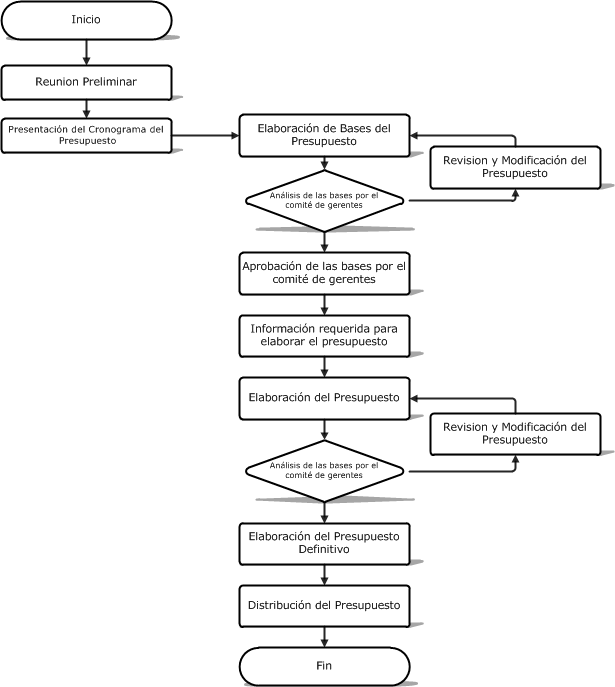
\includegraphics[angle=0,width=150mm]{img/dia/Presupuesto_General_tab_b.png}
		    \caption{Elaboraci\'on del Presupuesto GST}
		    \label{luna}
		\end{figure}
  
% \begin{tikzpicture}
% [auto, node distance = 1cm and -1cm,
%  every node/.style = {%
%   draw = black, thick, fill = white!50,inner sep = 3pt, text badly centered},
%  rectangulo/.style = {%
%   rectangle, text width=2.5cm, minimum size = 1.5cm},
%  rectanguloredo/.style = {rectangle, rounded corners = 10pt},
%  line/.style = {draw, thick, -latex,shorten >=1pt},
% ]
% 
%  \node (a) [rectanguloredo, text width=3.5cm, minimum size=1.2cm]
%   {Elaboraci\'on de Presupuesto};
%  \Paral[0.55]{a}
% %  \node (b) [rectangulo, below left=of a] {Presentacion del Cronograma de Presupuestos};
% %  \Paral{b} 
%  \node (b) [rectangulo, below =of a, text width=4cm] {Reuni\'on Preliminar};
%  \Paral{b} 
%  \node (c) [rectangulo, below =of b, text width=4cm] {Presentaci\'on del Cronograma del Presupuesto};
%  \Paral{c}
%  
%  \node (d) [rectangulo, below =1cm of c, text width=4cm] {Elaboracion de las bases del Presupuesto};
%  
%  \node (e) [rectangulo,below= 3.5cm of c ,right =3cm , text width=4cm] {Revisi\'on , Modificaci\'on};
%  \Paral{e}
% %  \node (e) [rectangulo, below =of c, text width=2.2cm] {informacion requerida para elab el Presupuesto};
% %  \Paral{e}
%  \node (f) [diamond, below =.5cm of d, text width=2cm] {An\'alisis Aprobacion-Gerencial};
%  \Paral{f}
% %  \node (g) [regular polygon, regular polygon sides=4, below = of f, text width=1cm] 
% %   {Si o no};
%  \node (g) [rectangulo, below = .5cm of f, text width=4cm] 
%   {informaci\'on requerida para elaborar el Presupuesto };
% 
%  \node (h) [diamond, below =2.5cm of f, text width=2cm] {Analisis y ajustes por parte de los Gerentes};
%  \Paral{h}
%  
%  \node (i) [rectangulo, below= of g ,right =3cm , text width=4cm] {Revisi\'on , Modificaci\'on};
%  
%  \node (j) [rectanguloredo, below = of h, rounded corners = 10pt, text width=4cm,  
%   minimum size=1cm] {Distribucion de Presupuesto};
%   
% % \newdimen\midima
% % \pgfextractx{\midima}{(a.south)}
% % \newdimen\midimb
% % \pgfextractx{\midimb}{(b.north)}
% % \newdimen\midimc
% % \pgfextractx{\midimc}{(c.north)}
% % \newdimen\midimd
% % \pgfextractx{\midimd}{(d.west)}
% % \newdimen\midime
% % \pgfextractx{\midime}{(e.south)}
% % \newdimen\midimf
% % \pgfextractx{\midimf}{(f.north)}
% % \newdimen\midimaw
% % \pgfextractx{\midimaw}{(a.west)}
% % \newdimen\midimgw
% % \pgfextractx{\midimgw}{(g.west)}
% 
%  \begin{scope}[every path/.style=line]
%  \path
%   (a.south) -- ++(0,-0.4) |- ++($(\midimb,0)-(\midima,0)$) -| (b.north);
% %  \path
% %   (b.south) -- ++(0,-0.4) |- ++($(\midimc,0)-(\midima,0)$) -| (c.north);
%  \path (b) -- (c);
% %  \path (c) -- (d);
% 
% %  \path
% %   (d.south) -- ++(0,-0.4) |- ++($(\midimd,0)-(\midimf,0)$) -| (f.east);
% 
% %  \path
% %   (e.south) -- ++(0,-0.4) |- ++($(\midime,0)-(\midimf,0)$) -| (f.north);
% %   \path (d.south) -- (f.east);
% %  \path (f) -- (g);
% %  \path (g.west) node[draw = none, fill = none, yshift = 0.3cm, xshift = -0.4cm] {text} 
% %   -- ++(-3.5,0) -- ++($(0,\midimaw)-(0,\midimgw)$) |- (a);
% %  \path (g) -- node[draw = none, fill = none, xshift = 0.1cm] {text} (h);
%  \end{scope}
% \end{tikzpicture}
	\end{center}
  \end{subsection}
 
	\newpage
	
	\begin{itemize}
	\item[\ding{229}]{}

	\begin{itemize}
	    \item[\ding{237}]{...
	%imagenes only 3 figures are allowed per page
		\begin{figure}[htb]
		    \centering
		    \includegraphics[angle=0,width=4mm]{moon.png}
		    \caption{caption}
		    \label{luna}
		\end{figure}
	    }
	\end{itemize}

	\begin{itemize}
	    \item[\ding{237}]{...
		\begin{figure}[htb]
		    \centering
		    \includegraphics[angle=0,width=4mm]{moon.png}
		    \caption{caption}
		    \label{luna}
		\end{figure}
	    }
	\end{itemize}

	\begin{figure}[htb]
	    \centering
	    \includegraphics[angle=0,width=4mm]{moon.png}
	    \caption{caption}
	    \label{luna}
	\end{figure}

	
	%lista
	\begin{itemize}
	\item[\ding{182}]{ list \ding{231} \includegraphics[angle=0,width=4mm]{moon.png}}
	\end{itemize}
    \end{itemize}
%     \vfill{\hrule
% 	\vspace{5mm}
% 	\textsuperscript{*} Example ...
%     }
  \end{section}


  \newpage
  \begin{section}
  {\color{kblue} Cronograma}

    \begin{subsection}
    {\color{kgreen}subsection ...}
    \end{subsection}

    \begin{subsubsection}
    {\color{kgray}Sub---subsection ...}
    \end{subsubsection}

    \begin{itemize}
	\item[\ding{229}]{...}

	\begin{itemize}
	    \item[\ding{237}]{...
	%imagenes only 3 figures are allowed per page
		\begin{figure}[htb]
		    \centering
		    \includegraphics[angle=0,width=4mm]{moon.png}
		    \caption{caption}
		    \label{luna}
		\end{figure}
	    }
	\end{itemize}

	\begin{itemize}
	    \item[\ding{237}]{...
		\begin{figure}[htb]
		    \centering
		    \includegraphics[angle=0,width=4mm]{moon.png}
		    \caption{caption}
		    \label{luna}
		\end{figure}
	    }
	\end{itemize}

	\begin{figure}[htb]
	    \centering
	    \includegraphics[angle=0,width=4mm]{moon.png}
	    \caption{caption}
	    \label{luna}
	\end{figure}
	
	\footnotesize{\scshape{
	  \begin{invoice}{MXN}{0}
	    \ProjectTitle{\color{red}Costos por Unidad de Negocio}%
	    
	    \Fees{s  Por 4 Modulos}{ .... }{}
	    \Fee{...}{2000}{1}
	    \Fee{...}{2000}{1}
% 	    \Fee{Control Unidades Fuera de la Ciudad}{2000}{1}
% 	    \Fee{Control de Unidades en Servicio}{2000}{1}
% 	    \Fee{Servidor 1 a\~no 24-hrs/365-dias}{2000}{1}
% 	    \Discount{1 Modulo Gratis}{2000}
	  \end{invoice}
	    }%end of size
	  }%end of smallcaps
	  
	%lista
	\begin{itemize}
	\item[\ding{182}]{ list \ding{231} \includegraphics[angle=0,width=4mm]{moon.png}}
	\end{itemize}
    \end{itemize}
%     \vfill{\hrule
% 	\vspace{5mm}
% 	\textsuperscript{*} Example ...
%     }
  \end{section}

\newpage

  \begin{section}
  {\color{kblue} Bases Fundamentales}

    \begin{subsection}
    {\color{kgreen}Recopilar informacion de las Unidades de Negocio}
    \end{subsection}

    \begin{subsubsection}
    {\color{kgray}Delegar Responsabilidades ...}
    \end{subsubsection}

    \begin{itemize}
	\item[\ding{229}]{...}

	\begin{itemize}
	    \item[\ding{237}]{...
	%imagenes only 3 figures are allowed per page
		\begin{figure}[htb]
		    \centering
		    \includegraphics[angle=0,width=4mm]{moon.png}
		    \caption{caption}
		    \label{luna}
		\end{figure}
	    }
	\end{itemize}

	\begin{itemize}
	    \item[\ding{237}]{...
		\begin{figure}[htb]
		    \centering
		    \includegraphics[angle=0,width=4mm]{moon.png}
		    \caption{caption}
		    \label{luna}
		\end{figure}
	    }
	\end{itemize}

	\begin{figure}[htb]
	    \centering
	    \includegraphics[angle=0,width=4mm]{moon.png}
	    \caption{caption}
	    \label{luna}
	\end{figure}
	
	\footnotesize{\scshape{
	  \begin{invoice}{MXN}{0}
	    \ProjectTitle{\color{red}Costos por Unidad de Negocio}%
	    
	    \Fees{s  Por 4 Modulos}{ .... }{}
	    \Fee{...}{2000}{1}
	    \Fee{...}{2000}{1}
% 	    \Fee{Control Unidades Fuera de la Ciudad}{2000}{1}
% 	    \Fee{Control de Unidades en Servicio}{2000}{1}
% 	    \Fee{Servidor 1 a\~no 24-hrs/365-dias}{2000}{1}
% 	    \Discount{1 Modulo Gratis}{2000}
	  \end{invoice}
	    }%end of size
	  }%end of smallcaps
	  
	%lista
	\begin{itemize}
	\item[\ding{182}]{ list \ding{231} \includegraphics[angle=0,width=4mm]{moon.png}}
	\end{itemize}
    \end{itemize}
%     \vfill{\hrule
% 	\vspace{5mm}
% 	\textsuperscript{*} Example ...
%     }
  \end{section}
%%%%%%%%%%%%%%%%%%%%%%%%%%%%%%%%%%%%%%%%%%%%%%%%%%%%%


  %%% Squeleton %%%
%   \begin{section}
%   {\color{kblue} Section...}
% 
%     \begin{subsection}
%     {\color{kgreen}subsection ...}
%     \end{subsection}
% 
%     \begin{subsubsection}
%     {\color{kgray}Sub---subsection ...}
%     \end{subsubsection}
% 
%     \begin{itemize}
% 	\item[\ding{229}]{...}
% 
% 	\begin{itemize}
% 	    \item[\ding{237}]{...
% 	%imagenes only 3 figures are allowed per page
% 		\begin{figure}[htb]
% 		    \centering
% 		    \includegraphics[angle=0,width=4mm]{moon.png}
% 		    \caption{caption}
% 		    \label{luna}
% 		\end{figure}
% 	    }
% 	\end{itemize}
% 
% 	\begin{itemize}
% 	    \item[\ding{237}]{...
% 		\begin{figure}[htb]
% 		    \centering
% 		    \includegraphics[angle=0,width=4mm]{moon.png}
% 		    \caption{caption}
% 		    \label{luna}
% 		\end{figure}
% 	    }
% 	\end{itemize}
% 
% 	\begin{figure}[htb]
% 	    \centering
% 	    \includegraphics[angle=0,width=4mm]{moon.png}
% 	    \caption{caption}
% 	    \label{luna}
% 	\end{figure}
% 	
% 	\footnotesize{\scshape{
% 	  \begin{invoice}{MXN}{0}
% 	    \ProjectTitle{\color{red}Costos para la Unidad de Negocio}%
% 	    
% 	    \Fees{s  Por 4 Modulos}{ .... }{}
% 	    \Fee{...}{2000}{1}
% 	    \Fee{...}{2000}{1}
% % 	    \Fee{Control Unidades Fuera de la Ciudad}{2000}{1}
% % 	    \Fee{Control de Unidades en Servicio}{2000}{1}
% % 	    \Fee{Servidor 1 a\~no 24-hrs/365-dias}{2000}{1}
% % 	    \Discount{1 Modulo Gratis}{2000}
% 	  \end{invoice}
% 	    }%end of size
% 	  }%end of smallcaps
% 	  
% 	%lista
% 	\begin{itemize}
% 	\item[\ding{182}]{ list \ding{231} \includegraphics[angle=0,width=4mm]{moon.png}}
% 	\end{itemize}
%     \end{itemize}
%     \vfill{\hrule
% 	\vspace{5mm}
% 	\textsuperscript{*} Example ...
%     }
%   \end{section}

 }% end of serif font family

\end{document}
